\documentclass[12pt]{article}
\usepackage[utf8]{inputenc}
\usepackage{amsmath, amsfonts}
\usepackage{hyperref}
\usepackage[table]{xcolor}
\usepackage{xcolor}
\usepackage{booktabs}
\usepackage{tikz, pgfplots}
\pgfplotsset{compat=newest}

\title{Using Conjugate Gradient to Solve Matrix Equation}
\author{Xinyu Chen}
\date{\today}

\begin{document}

\begin{table}[h]
\centering\footnotesize
\begin{tabular}{l|c|c|c|c|c}
\toprule
& Feb. 22 & Feb. 23 & Feb. 24 & Feb. 25 & Feb. 26 \\
\midrule
\textbf{Wiki} & \cellcolor{cyan} & \cellcolor{white} & \cellcolor{white} & \cellcolor{white} & \cellcolor{white} \\
\hline
\hline
\hline
\hline
\hline
\textbf{xxx} & & & & \cellcolor{cyan} & \\
\bottomrule
\end{tabular}
\end{table}

\maketitle

\section{System of Linear Equations}

One simple example could be a system of linear equation $\boldsymbol{A}\boldsymbol{{x}}=\boldsymbol{b}$ such that
\begin{equation}
\boldsymbol{A}=\begin{bmatrix}
4 & 1 \\
1 & 3 \\
\end{bmatrix},\quad\boldsymbol{b}=\begin{bmatrix}
1 \\
2 \\
\end{bmatrix}
\end{equation}
This case consists of two linear equation, and it can also be written as follows,
\begin{equation}
\left\{
\begin{aligned}
4x_1+x_2=1 \\
x_1+3x_2=2 \\
\end{aligned}
\right.
\end{equation}
where the exact solution is
\begin{equation}
\boldsymbol{x}=\begin{bmatrix}
x_1 \\
x_2 \\
\end{bmatrix}=\begin{bmatrix}
1/11 \\
7/11 \\
\end{bmatrix}\approx\begin{bmatrix}
0.0909 \\
0.6364 \\
\end{bmatrix}
\end{equation}

Figure~\ref{example1} shows the system of linear equations in an $x-y$ axis.

\begin{figure}[h]
    \centering
    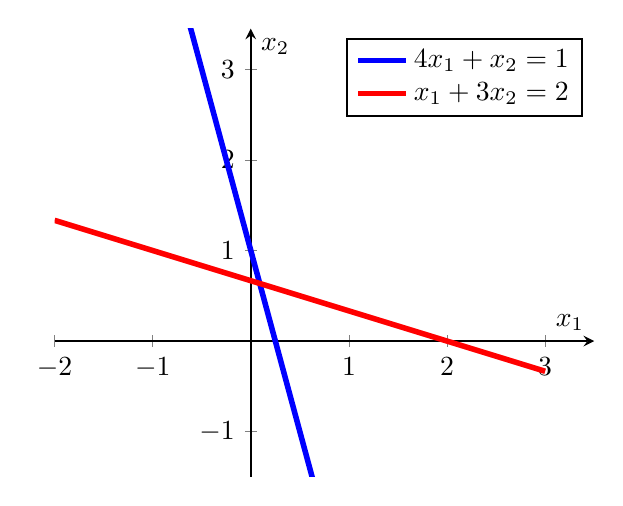
\begin{tikzpicture}
\begin{axis}[axis lines=middle, line width=0.7, enlargelimits=upper, domain=-2:3, ymin=-1.5, ymax=3, xlabel=$x_1$, ylabel=$x_2$, legend entries={{$4x_1+x_2=1$}, {$x_1+3x_2=2$}}]
\addplot [smooth, color=blue, line width = 2] {1-4*x};
\addplot [smooth, color=red, line width = 2] {(2-x)/3};
\end{axis}
\end{tikzpicture}
    \caption{Illustration of the system of linear equations.}
    \label{example1}
\end{figure}

% Figure~\ref{example2}

\begin{figure}[h]
    \centering
    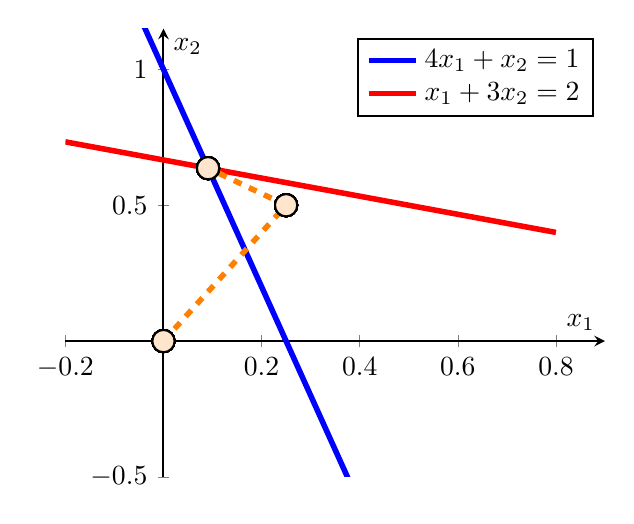
\begin{tikzpicture}
\begin{axis}[axis lines=middle, line width=0.7, enlargelimits=upper, domain=-0.2:0.8, ymin=-0.5, ymax=1, xlabel=$x_1$, ylabel=$x_2$, legend entries={{$4x_1+x_2=1$}, {$x_1+3x_2=2$}}]
\addplot [smooth, color=blue, line width = 2] {1-4*x};
\addplot [smooth, color=red, line width = 2] {(2-x)/3};
\addplot[only marks, mark size=4, color=orange!20, draw=black] (0,0);
\addplot[only marks, mark size=4, color=orange!20, draw=black] (0.25,0.5);
\addplot[only marks, mark size=4, color=orange!20, draw=black] (0.09090909,0.63636364);
\addplot[color=orange, dashed, line width = 2] coordinates {(0,0) (0.25,0.5) (0.09090909,0.63636364)};
\end{axis}
\end{tikzpicture}
    \caption{Illustration of the system of linear equations.}
    \label{example2}
\end{figure}

For the Lyapunov equation:
\begin{equation}
\boldsymbol{A}\boldsymbol{X}+\boldsymbol{X}\boldsymbol{A}^\top=\boldsymbol{W}
\end{equation}
with
\begin{equation}
\boldsymbol{A}=\begin{bmatrix}
-2 & -1 \\
-1 & 0 \\
\end{bmatrix},\quad\boldsymbol{W}=\begin{bmatrix}
-1 & 0 \\
0 & -1 \\
\end{bmatrix}
\end{equation}


\end{document}
